\documentclass[10pt, aspectratio=169, compress]{beamer}
\usetheme[progressbar=frame title, numbering=fraction]{metropolis}      % Use metropolis theme 
\setbeamertemplate{section in toc}[sections numbered]
\setbeamertemplate{subsection in toc}[subsections numbered]
\useoutertheme[subsection=false]{miniframes}
\setbeamercolor{section in head/foot}{fg=white, bg=mDarkTeal}
\setbeamercolor{background canvas}{bg=white}
\setbeamerfont{section in head/foot}{series=\bfseries}

\usefonttheme[onlymath]{serif}
\usepackage{amsmath}
\RequirePackage{silence}
\WarningFilter{remreset}{The remreset package}
\usepackage{ragged2e}
\usepackage{booktabs}
\usepackage{makecell}
\usepackage{float}
\usepackage{subfig}
\usepackage{tikz}
\usetikzlibrary{positioning,calc,trees}
\usepackage[flushleft]{threeparttable}	% 3 part table 
\usepackage[justification=centering]{caption}
\captionsetup{skip=0pt}
\graphicspath{{./fig/}}

% colors
\usepackage{colortbl}
\usepackage{url}
\urlstyle{rm}
\definecolor{darkblue}{rgb}{0,0,.4}

\makeatletter
\let\beamer@writeslidentry@miniframeson=\beamer@writeslidentry
\def\beamer@writeslidentry@miniframesoff{%
	\expandafter\beamer@ifempty\expandafter{\beamer@framestartpage}{}% does not happen normally
	{%else
		% removed \addtocontents commands
		\clearpage\beamer@notesactions%
	}
}
\newcommand*{\miniframeson}{\let\beamer@writeslidentry=\beamer@writeslidentry@miniframeson}
\newcommand*{\miniframesoff}{\let\beamer@writeslidentry=\beamer@writeslidentry@miniframesoff}
\beamer@compresstrue
\makeatother

%==============================================================
% Title Page
%==============================================================
%Information to be included in the title page:
\title{Exportando tablas en Stata III}
\subtitle{Replicación de Papers}
\author{Rony Rodriguez-Ramírez} 
\institute{LAMBDA}
\titlegraphic{\hfill
\includegraphics[height=1.5cm]{dime}}
\date{\today}
%==============================================================
\begin{document}
%------------------------------------------------	
\begin{frame}[plain]
	\maketitle 
\end{frame}
%------------------------------------------------
\section{Intro to Git}
%-----------------------------------------------
\subsection{Intro to Git}
%-----------------------------------------------
\begin{frame}
	\frametitle{Antes de la sesion:}

	\begin{itemize}
		\item Confirmemos que tienes una cuenta en GitHub: \hyperlink{https://github.com/join}{https://github.com/join}
		\item Instalar GitKraken: \hyperlink{https://www.gitkraken.com/}{https://www.gitkraken.com/}
	\end{itemize}
\end{frame}
%-----------------------------------------------
\begin{frame}
	\frametitle{Intro to Git}	
	\begin{figure}[H]
		\centering
		
\includegraphics[width=0.35\textwidth]{finaldoc.pdf}
	\end{figure}
\end{frame}
%-----------------------------------------------
\begin{frame}
	\frametitle{¿Por qué Git?}

	\begin{itemize}
		\item Nos permite hacer rastreo de una documento. 
		\item ¿Quién lo hizo? ¿Qué modificaciones pasaron? ¿Por qué se hicieron estos cambios?
		\item Nos facilita colaboración entre personas.
		\item Podemos eliminar el problema de ``copia conflictiva'' en Dropbox. 
		\item Podemos configurar nuestro flujo de trabajo para replicaciones.
	\end{itemize}
\end{frame}
%-----------------------------------------------
\begin{frame}
	\frametitle{Intro to Git}

	Tres conceptos claves en Git:

	\begin{itemize}
		\item Clonar (Clone)
		\item Cometer (Commit)
		\item Rama (Branch)
	\end{itemize}
\end{frame}
%-----------------------------------------------
\begin{frame}
	\frametitle{¿Qué es clonar}

	Clonar es similar a descargar un repositorio en su computadora

	La diferencia entre clonar y descargar radica en que Git clona una repositorio y recuerda de donde se ha descargado este repositorio. Esto es necesario ya que Git conoce donde se debe compartir las ediciones que se hacen a una archivo específico de una repositorio.
\end{frame}
%-----------------------------------------------
\begin{frame}
	\frametitle{Clonar un repositorio}

	\begin{center}
		¿Cómo clonar un repositorio? \\ Live Preview
	\end{center}
	
\end{frame}
%-----------------------------------------------
\begin{frame}
	\frametitle{Explorando el clon}

	Dos puntos a tomar en cuenta en torno a los repositorios: 

	\begin{itemize}
		\item Commits
		\item Branches
	\end{itemize}

\end{frame}
%-----------------------------------------------
\begin{frame}
	\frametitle{¿Qué es una commit?}

	\begin{itemize}
		\item En lugar de tener una lista de cada versión guardada de un archivo, en Git usamos commits para indicar cuál es cada diferencia significativa entre dos versiones de nuestra carpeta de proyecto.
		\item Cada commit es una snapshot de todos los archivos de un proyecto. Git lista cada snapshot y lo compara con el snapshot anterior.
		\item Cada commit tiene una tiempo y rastreo de quién hizo el commit.  
	\end{itemize}

\end{frame}
%-----------------------------------------------
\begin{frame}
	\frametitle{¿Como hacer un commit?}

	\begin{center}
		Live Preview
	\end{center}

\end{frame}
%-----------------------------------------------
\begin{frame}
	\frametitle{Introduciendo branches (ramas)}

	\begin{columns}
		\begin{column}{0.5\textwidth}
			\begin{itemize}
				\item Branc es la \textbf{\textit{característica clave}} clave de Git.
				\item Las ramas nos permite crea una copia del código donde nosotros podemos experimentar. Si nos gusta el resultado podemos unir nuestro experimento con el projecto principal.
			\end{itemize}
		\end{column}
		\begin{column}{0.5\textwidth}
			\begin{center}
			 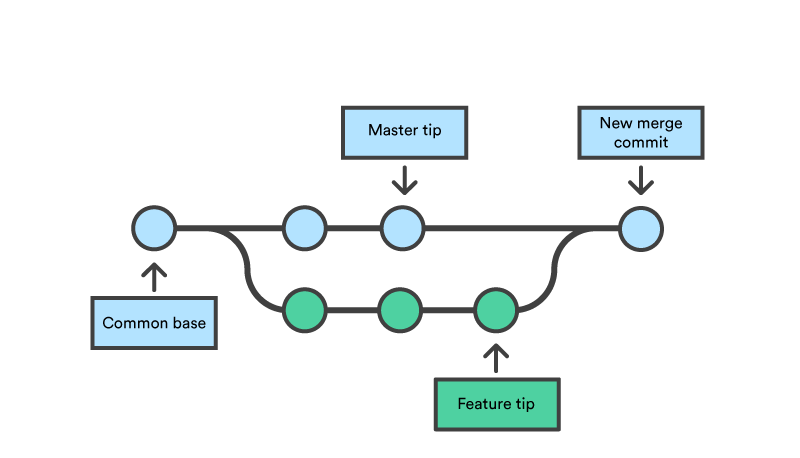
\includegraphics[width=1\textwidth]{git.png}
			 \end{center}
		\end{column}
	\end{columns}

\end{frame}
%-----------------------------------------------
\begin{frame}
	\frametitle{Más materiales}

	\begin{itemize}
		\item Lamentablemente por tiempo no podremos introducir más features de Git. 
		\item En cavas podrás encontrar más materiales.
	\end{itemize}
\end{frame}
%-----------------------------------------------
\section{Regresión discontinua}
\subsection{Regresión discontinua}
%-----------------------------------------------
\begin{frame}
	\frametitle{Intro: RDD}

	\begin{itemize}
		\item Presentado por primera vez para estudiar el impacto del reconocimiento al mérito por Thistlethwaite \& Campbell (1960).
		\item Sin embargo, solo comenzó a llamar la atención en economía desde finales de la década de 1990.
		\item Pero ¿qué es una discontinuidad?
		\begin{itemize}
			\item Una ruptura brusca en los valores de una función.
			\item Matemáticamente, estamos hablando de una ecuación por partes (piecewise equation):
			$$
			f(x) = \left\{
			\begin{array}{ll}
			\frac{1}{2} x, 	& \quad x < 5 \\
			2+\frac{1}{2}x,  & \quad x \geq 5
			\end{array}
			\right.
			$$
		\end{itemize}
	\end{itemize}
\end{frame}
%-----------------------------------------------
\begin{frame}
	\frametitle{Uso de RDD}

	\begin{itemize}
		\item No tenemos un RCT y nos preocupan las variables endógenas.
		\item RDD utiliza la asignación de discontinuidad exógena para estimar los efectos causales; es decir, las observaciones de un lado de la ruptura terminan siendo muy similares a las del otro lado.
		\item Esencialmente, terminamos con grupos equilibrados pero no tenemos una asignación de tratamiento aleatorizada.
	\end{itemize}

\end{frame}
%-----------------------------------------------
\begin{frame}
	\frametitle{Prinicipios de RDD}

	Randomización local: 

	\begin{itemize}
		\item El estado de tratamiento es una función determinista de una variabla $a$, por lo cual cuando conocemos $X$ conocemos el estado de tratamiento $D_x$. 
		\item El estado de tratamiento es una función discontinua de $a$ porque no importa que tan cerca X llegue al corte, $D_x$ continua sin cambios hasta que el corte se ha alcanzado.
		$$
		D_x = 
		\begin{cases}
		1 &\text{if}~X \geq \text{cutoff} \\  
		0 &\text{if}~X < \text{cutoff} 
		\end{cases}
		$$
	\end{itemize}

\end{frame}
%-----------------------------------------------
\begin{frame}
	\frametitle{Prinicipios de RDD}

	\begin{itemize}
		\item Llamamos a nuestra variable de asignación $X$, variable en ejecución (forcing or running variable).
		\item Un punto importante, es que esta variable no es ortogonal a:
		\begin{itemize}
			\item Las características observables de los individuos. 
			\item Las características no observables de los individuos.
		\end{itemize}
	\end{itemize}
	

\end{frame}
%-----------------------------------------------
\begin{frame}
	\frametitle{RD como una randomización local}

	\begin{figure}
		\centering
		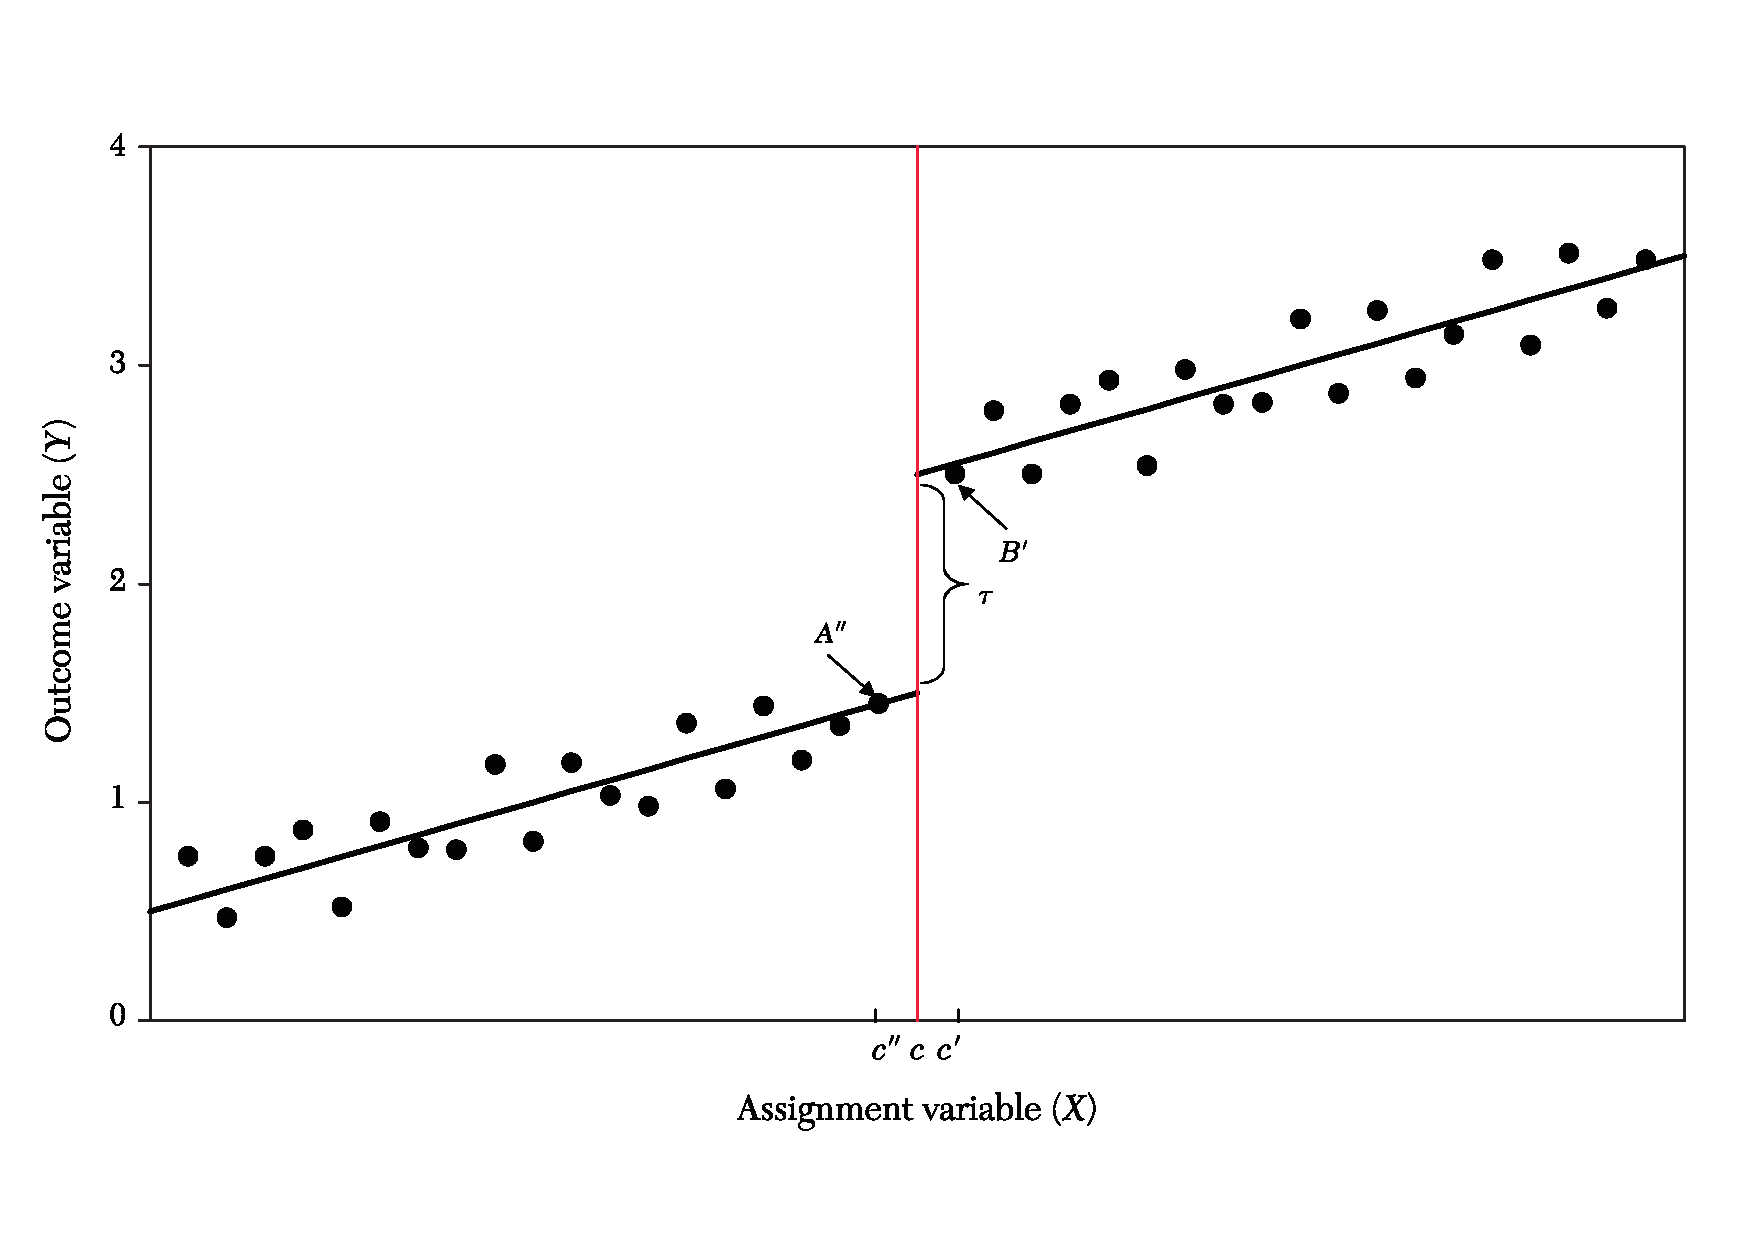
\includegraphics[width=0.7\textwidth]{rdd.pdf}
	\end{figure}

\end{frame}
%-----------------------------------------------
\begin{frame}
	\frametitle{Dos condiciones claves en RDDs}

	\begin{enumerate}
		\item El tratamiento en la población debe depender en que si la variable observada excede el valor crítico denota como $c$.
		\item Los individuos no tiene un control preciso de la variable de asignación.
		\begin{itemize}
			\item "Sin control preciso" significa que entre los que puntúan cerca del umbral, es cuestión de "suerte" en cuanto a qué lado del umbral aterrizan.
			\item Las personas que marginalmente pasan el corte o quedan atras, son asumidos como identicos (bastante similares).
		\end{itemize}
	\end{enumerate}

\end{frame}
%-----------------------------------------------

%==============================================================
\miniframesoff 	

\begin{frame}[plain, noframenumbering]
	\begin{center}
	\LARGE STATA TIME
		\begin{figure}[H]
			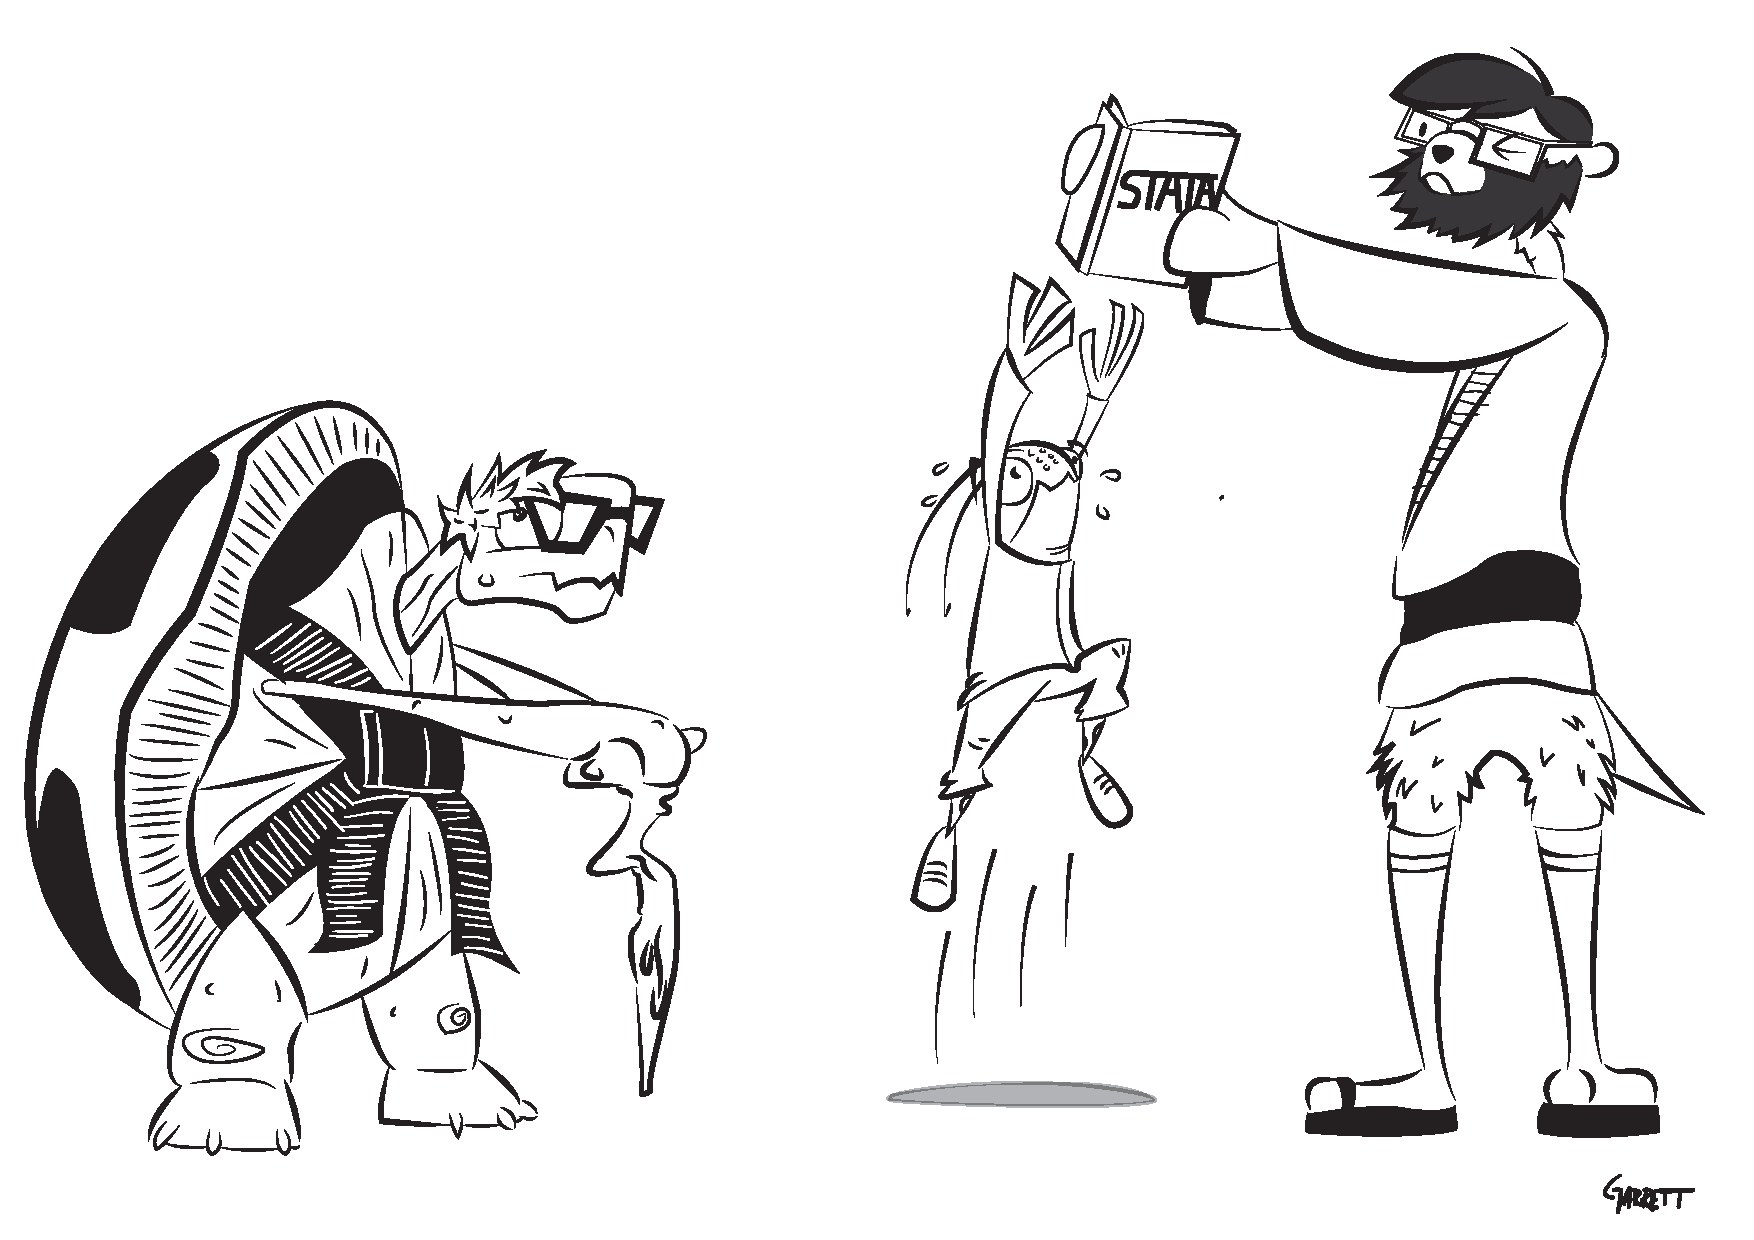
\includegraphics[width=0.57\textwidth]{stata.pdf}
		\end{figure}
	\end{center}
\end{frame}
%==============================================================
% END
%==============================================================	
\begin{frame}[plain, standout]
	Nos vemos mañana.
\end{frame}
%-----------------------------------------------
\end{document}		
